%%%
% Class 'kaobook' from https://github.com/fmarotta/kaobook
%
% Copyright (c) 2022 Antonio Coín Castro
%%%

\documentclass[
  a4paper,
	fontsize=11pt, % Base font size
	twoside=false, % Use different layouts for even and odd pages (in particular, if twoside=true, the margin column will be always on the outside)
	%open=any, % If twoside=true, uncomment this to force new chapters to start on any page, not only on right (odd) pages
	%chapterprefix=true, % Uncomment to use the word "Chapter" before chapter numbers everywhere they appear
	%chapterentrydots=true, % Uncomment to output dots from the chapter name to the page number in the table of contents
  secnumdepth=2,
	numbers=noenddot, % Comment to output dots after chapter numbers; the most common values for this option are: enddot, noenddot and auto (see the KOMAScript documentation for an in-depth explanation)
	%draft=true, % If uncommented, rulers will be added in the header and footer
	%overfullrule=true, % If uncommented, overly long lines will be marked by a black box; useful for correcting spacing problems
]{kaohandt}

% Choose the language
\ifxetexorluatex
	\usepackage{polyglossia}
	\setmainlanguage{spanish}
\else
	\usepackage[spanish]{babel} % Load characters and hyphenation
\fi

% Change default fonts
\setmathfont[range={\mathcal,\mathbfcal, \mathbb}]{NewCMMath-Regular.otf}

% Change page style
\pagestyle{scrheadings}

% Load the bibliography package
\usepackage[
  style=authoryear-comp,
  maxbibnames=99
]{kaobiblio}

% Add comma before year in citations
\renewcommand*{\nameyeardelim}{\addcomma\space}

% Bibliography side cite style
\renewcommand{\formatmargincitation}[1]{%
  \parencite{#1}: \citetitle{#1}.%
}

% Bibliography file
\addbibresource{bibliography.bib}

% Load the package for hyperreferences
\usepackage{kaorefs}


\DefineBibliographyStrings{spanish}{andothers={et~al\adddot}}

% Set reference colors
\hypersetup{
  pdfauthor = {Antonio Coín},
  pdftitle = {MCMC y la librería emcee},
  citecolor=teal,
  urlcolor=blue!50!black,
  %anchorcolor=OliveGreen,
  linkcolor=teal
}

% Load mathematical packages for theorems and related environments
\usepackage{kaotheorems}

% Set the paths where to look for images
\usepackage{subcaption}
\graphicspath{{img/}}

% Only show section titles in margintoc
\setcounter{margintocdepth}{\sectiontocdepth}

% Load additional packages
\usepackage{dsfont}  %\mathds

% Some custom commands
\newcommand{\R} {\ensuremath{\mathds{R}}}
\newcommand{\E} {\ensuremath{\mathds{E}}}
\newcommand{\eps}{\varepsilon}
\newcommand{\bm}{\symbf}

%% Scalar product
\newcommand\dotprod[2]{\left\langle #1,\, #2 \right\rangle}

\DeclareMathOperator{\var} {Var}
\DeclareMathOperator{\cov} {Cov}

% Do not re-initialize sidenote counter after each section
\counterwithout{sidenote}{section}

%%%%%%%%%%%%%%%
% DOCUMENT
%%%%%%%%%%%%%%%


\begin{document}

\title{Markov chain Monte Carlo y la librería emcee}
\author[FM]{Antonio Coín Castro}
\date{\normalsize{Julio 2022}}
\maketitle

\section{Problema a resolver}

Queremos obtener muestras de una distribución que no conocemos en forma cerrada\sidenote[][*-1]{También es posible que conozcamos \(p(x)\), pero que obtener muestras de ella directamente sea difícil computacionalmente.}, pero sí conocemos una función proporcional a su densidad. Formalmente, queremos muestrear de una densidad desconocida \(p(x)\) a través de una función conocida \(f(x)\), dado que \(p(x) \propto f(x)\). Esta situación es común, por ejemplo, en inferencia bayesiana, donde la distribución a posteriori es muchas veces intratable debido a la constante de normalización, pero sí sabemos que \(posterior \propto prior \times likelihood\).

Cuando \(x \in \R\), podemos emplear algoritmos Monte Carlo de muestreo por rechazo o \textit{rejection sampling}, que se basan en muestrear uniformemente del área que encierra \(f(x)\) a través de otra función auxiliar que recubre este área. Sin embargo, en dimensión superior estos algoritmos sufren rápidamente la llamada \textit{maldición de la dimensionalidad}. Es por esto que para muestrear de distribuciones multidimensionales surgen nuevos métodos: los algoritmos de Markov chain Monte Carlo (MCMC).

\begin{marginfigure}[*-9]
  \centering
  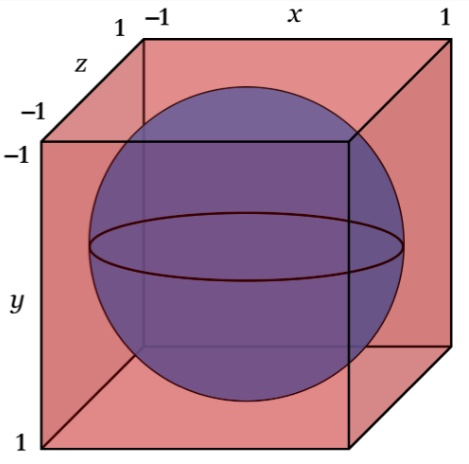
\includegraphics[width=.6\textwidth]{img/cube_sphere}
  \caption*{Intuitivamente, para recubrir el volumen de \(f(x)\) en dimensión alta necesitamos un volumen que escala exponencialmente con la dimensión.}
\end{marginfigure}

\section{MCMC}

Estos métodos se basan en la construcción iterativa de una cadena de Markov cuya distribución estacionaria es la distribución objetivo \(p(x)\). De esta forma, en una cadena suficientemente avanzada podemos tomar los distintos estados por los que se ha pasado como muestras aproximadas de \(p(x)\). A la hora de construir las cadenas, las probabilidades de transición se asignan de forma que se favorezcan regiones donde se acumula más densidad de la distribución objetivo (evaluando la función \(f(x)\) conocida). \marginnote[*-4]{Se consigue paliar un poco el problema de la maldición de la dimensionalidad, e incluso se puede reducir más la influencia de la dimensión controlando el tamaño de los pasos en la cadena.}

A diferencia de otros algoritmos de Monte Carlo, aquí obtenemos muestras correladas. Si se desean muestras i.i.d., se puede hacer \textit{thinning} de la traza y considerar solo una de cada \(n\) muestras.

\subsection{Algoritmo Metropolis-Hastings}

Se trata en realidad de un algoritmo marco (\sidecite[*-1]{metropolis1953equation}) a partir del cual han surgido muchos otros. Se basa en el uso de una distribución auxiliar simétrica\sidenote[][*2]{La función auxiliar se conoce como densidad propuesta o distribución de salto (\textit{proposal density} o \textit{jumping distribution}).} \(g(x'| x_t)\) que genera una propuesta para el estado siguiente a partir del estado actual (e.g. una distribución normal centrada en \(x_t\)). En cada iteración se genera una propuesta \(x'\), se calcula el \textit{ratio de aceptación} \(\alpha=f(x')/f(x_t)=p(x')/p(x_t)\), y finalmente se acepta el nuevo estado con probabilidad \(\min(1, \alpha)\). De esta forma se recorre aleatoriamente el espacio muestral, tendiendo a quedarse en las regiones de mayor densidad, y visitando ocasionalmente regiones poco probables con respecto a \(p(x)\).

\begin{figure}[h!]
  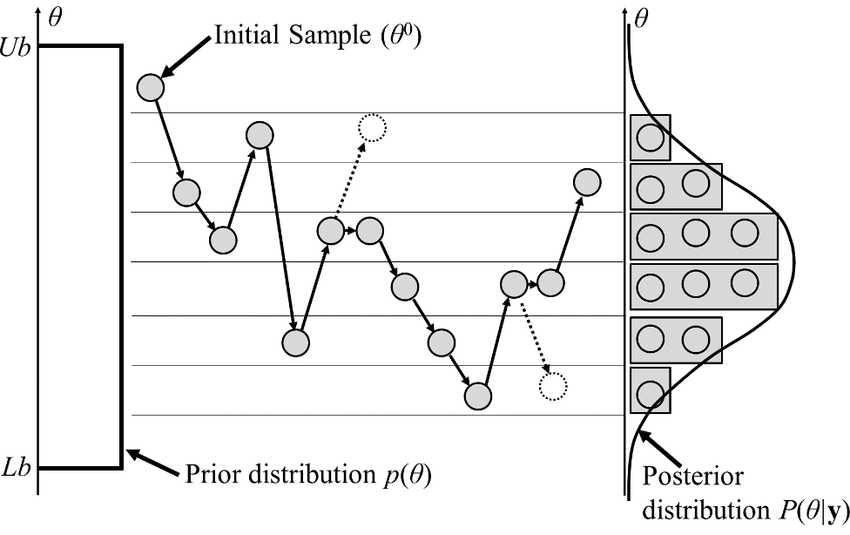
\includegraphics[width=.7\textwidth]{mh}
  \caption{Esquema del algoritmo Metropolis-Hastings~(extraída de \cite{jaewook2015metamodel}).}
\end{figure}

Una extensión directa es considerar distribuciones no simétricas para \(g\), donde el valor de \(\alpha\) se sustituye por
\[
\alpha=\frac{f(x')g(x_t \mid x')}{f(x_t)g(x'\mid x_t)},
\]
para que se sigan cumpliendo las ecuaciones de equilibrio de la cadena de Markov. Cabe destacar que cuando se rechaza una propuesta, se mantiene el estado anterior.

\subsection{Algoritmo de Gibbs}

Cuando el número de dimensiones es alto, encontrar una distribución de salto adecuada puede ser difícil (por ejemplo, puede ser necesario ajustar el tamaño del salto en cada dimensión individual). Un enfoque alternativo es el algoritmo de Gibbs (\sidecite[*-2]{geman1984stochastic}), que considera muestras separadas en cada dimensión. Concretamente, en cada paso se obtienen \textit{en orden} muestras unidimensionales (por ejemplo, mediante muestreo por rechazo) de cada variable mediante su distribución condicionada al resto de variables:
\[
p(x_k^{(i+1)} \mid x_{1}^{(i+1)}, \dots, x_{k-1}^{(i+1)}, x_{k+1}^{(i)}, \dots, x_L^{(i)}), \quad k=1,\dots,L.
\]
Notamos que usamos los valores más recientes de las variables disponibles en cada momento.

\subsection{Hamiltonian Monte Carlo}

Esta sub-familia de algoritmos introduce información del gradiente de la función objetivo para guiar la elección de propuestas de nuevos puntos. Se basan en la teoría de mecánica hamiltoniana, y en general consiguen aumentar la velocidad de convergencia debido a una elección inteligente de los nuevos puntos del espacio. Dentro de estos métodos destaca el \textit{No U-Turn Sampler} (NUTS, \sidecite[*-4]{hoffman2014no}), que tiene la ventaja añadida de que realiza un ajuste automático de hiperparámetros.

\subsection{Reversible-jump MCMC}

Estos métodos permiten variar la dimensionalidad subyacente del espacio muestral en cada propuesta (\sidecite[*0]{green1995reversible}). Teóricamente son útiles para muestrear de mixturas de gaussianas, procesos de Dirichlet o, en general, de cualquier distribución donde haya una variable latente que represente la dimensión del espacio. Sin embargo, no hay una implementación de referencia establecida.

\section{Affine-invariant ensemble sampler}

Una propiedad deseable de los algoritmos de muestreo es que sean \textit{invariantes por transformaciones afines}. Es decir, que vean dos distribuciones que difieren en una transformación afín, \(p(x)\) y \(p_{A, b}(Ax + b)\), como de igual dificultad. Esto es útil, por ejemplo, cuando uno tiene distribuciones muy asimétricas en las que es difícil encontrar un tamaño de paso que funcione bien en todas las dimensiones, pero que tras un reescalado se simplifican notablemente.

\begin{marginfigure}[*-6]
  \centering
  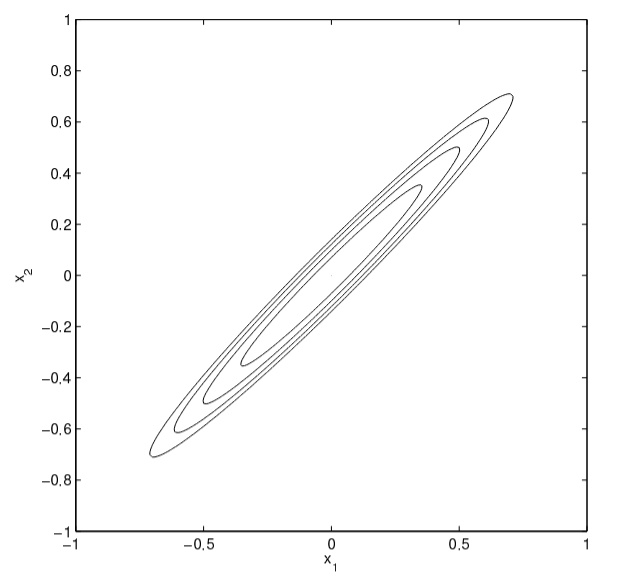
\includegraphics[width=.9\textwidth]{img/skewed}
  \caption*{Contornos de una distribución muy asimétrica en \(\R^2\).}
\end{marginfigure}

En general, un algoritmo de MCMC se puede describir como \(X(t+1)=R(X(t), \xi(t), p)\), donde \(X(t)\) es el estado de la cadena en el instante \(t\), \(p(x)\) es la distribución objetivo, y \(\xi(t)\) es una secuencia de variables aleatorias i.i.d. (asociadas a los procedimientos aleatorios de la cadena). La propiedad de invarianza afín se puede expresar como
\[
R(Ax+b, \xi(t), p_{A,b}) = AR(x, \xi(t), p) + b,
\]
para todo \(A, b\) y \(x\), y para casi todo \(\xi(t)\). Intuitivamente, esto quiere decir que si fijamos un generador aleatorio y ejecutamos dos veces el algoritmo, uno usando la densidad \(p\) empezando en \(X(0)\) y otro usando la densidad \(p_{A,b}\) con punto inicial \(Y(0)=AX(0)+b\), tendremos que \(Y(t)=AX(t)+b\).


En \sidetextcite[*-0.6]{goodman2010ensemble} los autores consideran un conjunto de cadenas (\textit{ensemble sampler}) con la propiedad de invarianza afín, inspirados en el algoritmo de optimización de Nelder-Mead. Específicamente, se tiene un conjunto \(X=(X_1, \dots, X_L)\) de \textit{walkers}, donde \(X_k(t)\) denota una cadena individual en el tiempo \(t\). En cada iteración, se usa una transformación invariante-afín contruida usando las posiciones \textit{actuales}\sidenote{En clara analogía con el algoritmo de Gibbs.} del resto de cadenas, mediante el llamado \textit{conjunto complementario}
\[
X_{-k}(t) = \{X_1(t+1), \dots, X_{k-1}(t+1), X_{k+1}(t), \dots, X_L(t)\}, \quad k=1,\dots, L.
\]

Para mantener la invarianza afín se hacen avanzar las cadenas de una en una y se utiliza un esquema Metropolis-Hastings de propuesta y aceptación para garantizar que se preserva la distribución conjunta del \textit{ensemble}. Se consideran principalmente dos tipos de movimientos:
\begin{itemize}
  \item \textit{Stretch move}. Para cada cadena \(1\leq k \leq L\) se elige aleatoriamente \(X_j \in X_{-k}(t)\), y la propuesta toma la forma
  \[
    X_k(t) \to Y = X_j + Z(X_k(t) - X_j),
  \]
  donde \(Z \stackrel{i.i.d.}{\sim} g(z)\) verificando\sidenote{Esta condición se impone para mantener la simetría de la propuesta.} \(g(z^{-1})=zg(z)\). Concretamente, se utiliza la densidad auxiliar parametrizada por \(a > 1\) dada por
  \[
  g(z) \propto \begin{cases}
    \frac{1}{\sqrt{z}}, & \text{si } z \in [a^{-1}, a],\\
    0, & \text{en otro caso.}
\end{cases}
  \]
  \begin{marginfigure}[*-1]
  \centering
  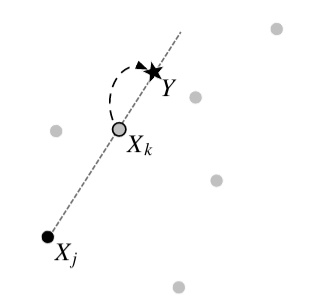
\includegraphics[width=.8\textwidth]{img/goodman_weare}
  \caption*{Esquema del \textit{stretch move} (extraído de \cite{goodman2010ensemble}).}
\end{marginfigure}

  La probabilidad de aceptación correspondiente para que se verifiquen las ecuaciones de equilibrio de las cadenas, suponiendo \(\R^N\) como espacio muestral, es
  \[
    \alpha = \min\left(1, \ Z^{N-1}\frac{p(Y)}{p(X_k(t))}\right).
  \]

  \item \textit{Walk move}. Para cada cadena \(1\leq k \leq L\) se elige un subconjunto aleatorio \(S_k \subseteq X_{-k}(t)\) con \(|S_k| \geq 2\), y se propone el movimiento
\[
X_k(t) \to Y = X_k(t) + W,
\]
donde \(W\) es una normal centrada en \(0\) y con la misma covarianza que la covarianza muestral de todas las cadenas de \(S_k\). La probabilidad de aceptación es directamente el ratio de aceptación de Metropolis, i.e., \(\min(1, p(Y)/p(X_k(t)))\).
\end{itemize}

\section{Librería emcee en Python}

El paquete \textit{emcee}\footnote[2]{\url{https://emcee.readthedocs.io/en/stable/}} de Python (\sidecite{foreman2013emcee}) proporciona una implementación paralela del algoritmo de \textcite{goodman2010ensemble}. La idea es dividir el conjunto de cadenas \(X\) en dos subconjuntos \(X^{(0)}\) y \(X^{(1)}\) de igual tamaño, y en cada iteración seguir un enfoque alternante de la siguiente forma:
\begin{enumerate}
  \item Se actualizan a la vez \textit{todas} las cadenas en \(X^{(0)}\) (mediante algunos de los movimientos disponibles, e.g. \textit{stretch move}) usando como conjunto complementario \(X^{(1)}\).
  \item Se utilizan las nuevas posiciones en \(X^{(0)}\) para actualizar \(X^{(1)}\).
\end{enumerate}
De esta forma se mantienen las ecuaciones de equilibrio de las cadenas, y cada uno de estos sub-pasos puede beneficiarse de un número arbitrario de procesadores\sidenote{Acotado superiormente por \(L/2\).} para su cómputo. También en el artículo citado se aconseja inicializar las cadenas en una bola gaussiana alrededor de un punto que se espere que tenga alta probabilidad según \(p(x)\).

Otra de las ventajas que ofrece este método frente a algoritmos clásicos es que solo requiere fijar unos pocos hiperparámetros (independientes de la dimensión subyacente), en lugar de los \(O(N^2)\) correspondientes, por ejemplo, a la matriz de covarianza de la distribución de salto \(N\)-dimensional en Metropolis-Hastings. Además, el paquete ha sido extendido para admitir otro tipo de movimientos paralelos, y el objetivo del proyecto es proporcionar un método de muestreo de propósito general que funcione correctamente en una clase amplia de problemas. Es muy usado por ejemplo en el campo de la astrofísica, y está bien establecido y testeado.

\printbibliography[title=Referencias]

\end{document}
